\begin{figure*}[hbtp]
  \centering
  \subfigure[Runtime in seconds (logarithmic scale) with \textit{Original Leiden}, \textit{igraph Leiden}, \textit{NetworKit Leiden}, and \textit{GVE-Leiden}]{
    \label{fig:leiden-compare--runtime}
    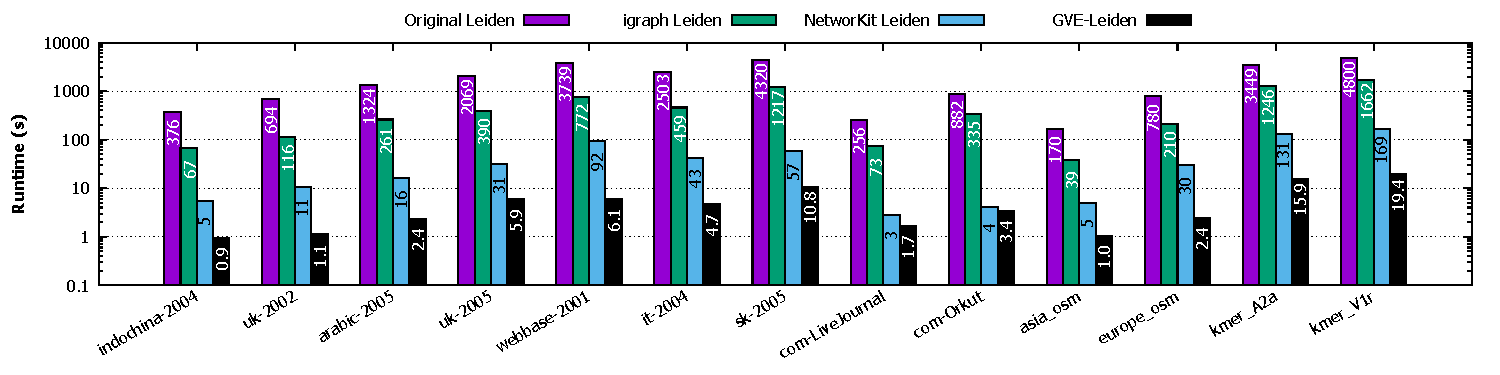
\includegraphics[width=0.98\linewidth]{out/leiden-runtime.pdf}
  } \\[-0ex]
  \subfigure[Speedup of \textit{GVE-Leiden} (logarithmic scale) with respect to \textit{Original Leiden}, \textit{igraph Leiden}, \textit{NetworKit Leiden}.]{
    \label{fig:leiden-compare--speedup}
    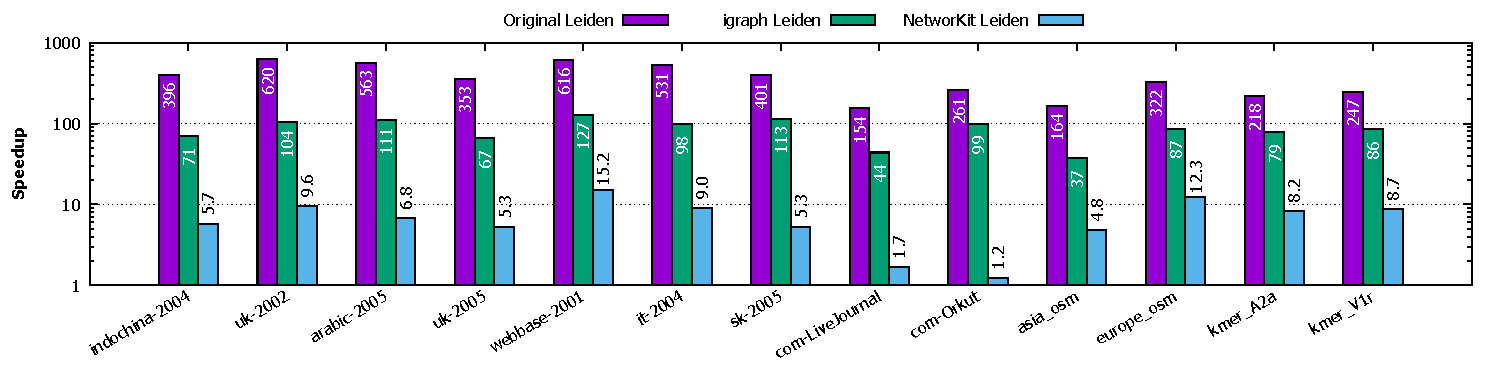
\includegraphics[width=0.98\linewidth]{out/leiden-speedup.pdf}
  } \\[-0ex]
  \subfigure[Modularity of communities obtained with \textit{Original Leiden}, \textit{igraph Leiden}, \textit{NetworKit Leiden}, and \textit{GVE-Leiden}.]{
    \label{fig:leiden-compare--modularity}
    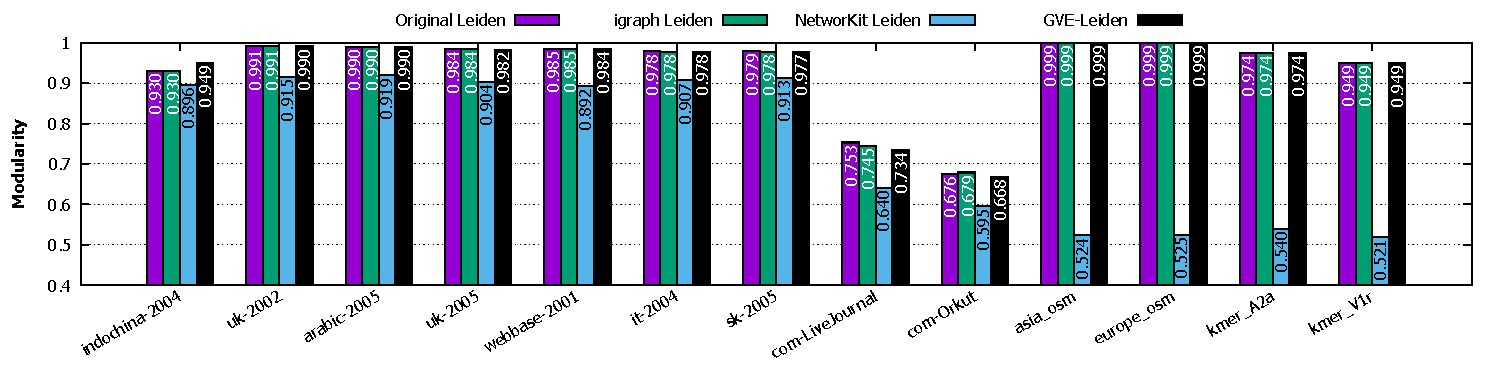
\includegraphics[width=0.98\linewidth]{out/leiden-modularity.pdf}
  } \\[-0ex]
  \subfigure[Fraction of disconnected communities (logarithmic scale) with \textit{Original Leiden}, \textit{igraph Leiden}, \textit{NetworKit Leiden}, and \textit{GVE-Leiden}.]{
    \label{fig:leiden-compare--disconnected}
    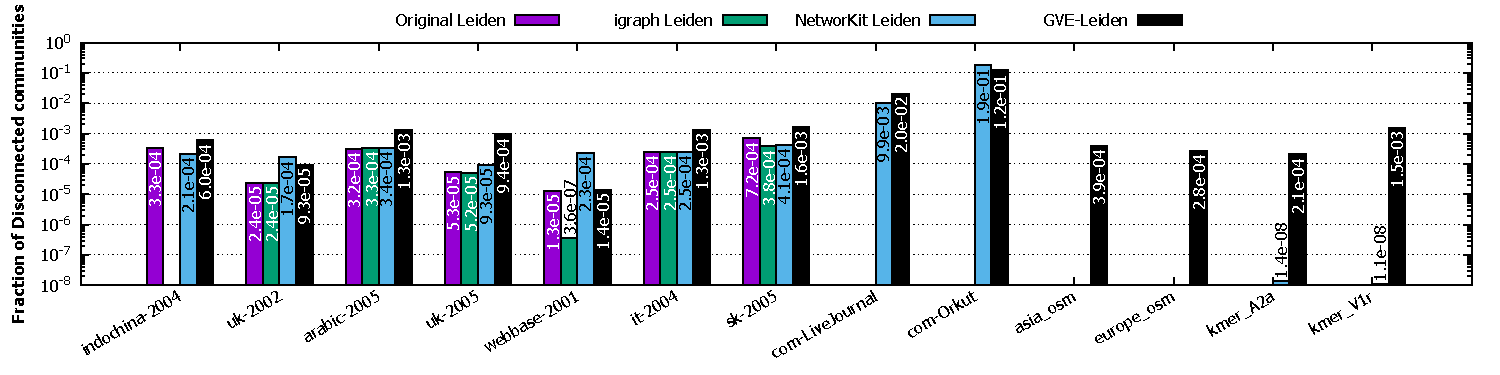
\includegraphics[width=0.98\linewidth]{out/leiden-disconnected.pdf}
  } \\[-2ex]
  \caption{Runtime in seconds (log-scale), speedup (log-scale), modularity, and fraction of disconnected communities (log-scale) with \textit{Original Leiden}, \textit{igraph Leiden}, \textit{NetworKit Leiden}, and \textit{GVE-Leiden} for each graph in the dataset.}
  \label{fig:leiden-compare}
\end{figure*}
